\documentclass[11pt,a4paper]{article}
\usepackage[left=2cm,right=2cm,top=2cm,bottom=3cm]{geometry}
\usepackage{amsmath,amsfonts,amsthm,amssymb,varioref,times}
\usepackage{gensymb}
\usepackage{tikz}
\usepackage{hyperref}
\hypersetup{
    colorlinks=true,
    linkcolor=blue,
    filecolor=magenta,      
    urlcolor=cyan,
}


%to resume numbering in a list
\usepackage{enumitem}

%pour ecrire en français avec les accents
\usepackage[utf8]{inputenc}
\usepackage[T1]{fontenc}
\usepackage{lmodern} % load a font with all the characters
\usepackage{units}

%Image-related packages
\usepackage{wrapfig}
\usepackage{float, graphicx}
\graphicspath{ {./img/} }
\usepackage{subcaption}
\usepackage[export]{adjustbox}


%pour faire des cadres
\usepackage{framed}
\usepackage{xcolor}
\usepackage{tcolorbox}

%chemistry frmulae
\usepackage{chemfig}
\usepackage{chemformula}
 

% parametres des entete et de pieds de pages
\usepackage{fancyhdr}
\pagestyle{fancy}
\fancyhf{}
\lhead{Exercice : Terminale}
\rhead{}
\chead{Ondes \& Vibration}
\rfoot{Page \thepage}
\lfoot{SZayyani}


% pour ecrire sur +sieurs colonnes
\usepackage{multicol}
\setlength{\columnseprule}{0.25pt}
\setlength{\columnsep}{60pt}

% Fusion de lignes de tableaux.
\usepackage{multirow}

% Position verticale des lettres dans la ligne de tableau.
\usepackage{array}


% MATH -----------------------------------------------------------
\newcommand{\To}{\longrightarrow}
\newcommand{\gpl}{\; g\cdot L^{-1}}
\newcommand{\gpmol}{\; g\cdot mol^{-1}}
\newcommand{\mpl}{\; mol\cdot L^{-1}}
\newcommand{\mps}{\; m\cdot s^{-1}}
\newcommand{\mpss}{\; m\cdot s^{-2}}
\newcommand{\es}[1]{\cdot10^{#1}}
\newcommand{\eng}[1]{\textcolor{purple}{= #1}}
\newenvironment{eg}
 {\begin{shaded} \textbf{Exemples:} } { \end{shaded}}

\newcounter{exo}
\newenvironment{exo}
 {\refstepcounter{exo} \begin{shaded}\noindent $\triangleright \quad$\textbf{Exercice: } } { \end{shaded}}    

\newenvironment{defn}[1]
 {\begin{leftbar}\noindent \textbf{Définition :\textit{ \quad #1} } } { \end{leftbar}} 
\newenvironment{rmrq}
 {\begin{shaded} \textbf{Remarque: Pour aller plus loin ...}\\ \itshape } { \end{shaded}}

\definecolor{shadecolor}{gray}{0.85}

\title{QCM - Ondes}
\date{}
\author{}

\setlength{\parindent}{0mm}
\setlength{\parskip}{2mm}

\begin{document}

\section*{Couche anti-réflet}

\begin{wrapfigure}{r}{0.5\textwidth}
    \centering
    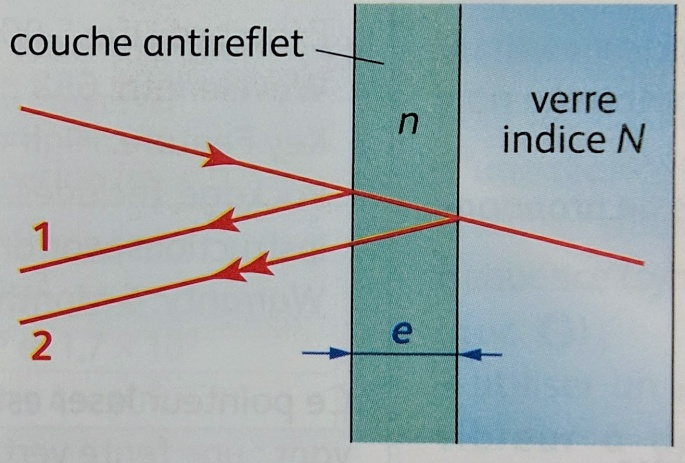
\includegraphics[widht=0.49\textwidth]{interfere.jpg}
\end{wrapfigure}
On utilise un laser de longueur d'onde dans le vide $\lambda_0=650\; nm$ pour éclairer l'intérieur d'une cuve dont les parois sont en verre d'indice de réfraction $N=1,5$. 
Pour éviter les réflexions du faisceau laser sur la face d'entrée du dispositif, on désire la recouvrir d'une couche anti-reflet dont l'indice de réfraction est $n = 1,35$. On souhaite déterminer l'épaisseur e de la couche transparente à appliquer sur le verre pour annuler la réflexion de la lumière du laser en incidence normale (rayons incidents perpendiculaires à la surface).
En effet, le second faisceau parcourt couche antireflet une distance plus importante que le premier car il effectue un aller-retour supplémentaire. Il en résulte une différence des retards entre les 1 deux faisceaux égale à:   $\Delta \tau = \dfrac{2Tne}{\lambda_0}$  avec $T$ la période de l’onde émise par le laser. 
Pour plus de lisibilité, les rayons ont été représentés légèrement inclinés par rapport à la normale sur la figure ci-dessus. 


Pour le laser utilisé, déterminer la plus petite valeur de e l’épaisseur e de cette couche anti-reflet. Montrer votre raisonnement, de manière précise, concise et rigoureuse à l’aide d’un calcul. 

\section*{Corrigé}

Pour éliminer les reflet il faut que les ondes réfléchies à la surface de la couche et celles réfléchies à l’intérieur de la couche soient en \textbf{opposition de phase}

c’est à dire il faut que $ \Delta\tau=( k+\dfrac{1}{2}) \cdot T$. 

Pour la couche la plus mince il faut prendre $k=0$, c’est à dire quand le \textbf{retard est la moitié de la période}: 
\text{car $T=\dfrac{d}{v}$}
\quad \text{Pour $k=0$}

\begin{align*}
    \Delta\tau &= ( k+\dfrac{1}{2}) \cdot T \\
        &= \dfrac{T}{2} \quad\quad \quad\quad \text{Pour $k=0$} \\
        &= \dfrac{2\cdot T\cdot n\cdot e}{\lambda_0} \quad \quad\quad\quad\quad\\
        \dfrac{T}{2} &=\dfrac{2\cdot T\cdot n\cdot e}{\lambda_0}\\
        e &= \dfrac{\lambda_0}{4\cdot n}\\ 
\end{align*} 
et donc applicaiton numérique : 
$$ e=\dfrac{650\es{-9}}{4(1,35)} = 120\; nm$$







\end{document}